\subsubsection{Klassen UserAccess}
Klassen UserAccess implementerer IUserAccess og står for at skrive og læse user records til/fra databasen.
UserAccess indeholer administrator funktionalitet til at slette alle users på databasen. Herudover står UserAccess for data editing af users samt validering af userdata før det gemmes.

\begin{figure}[h]
\centering
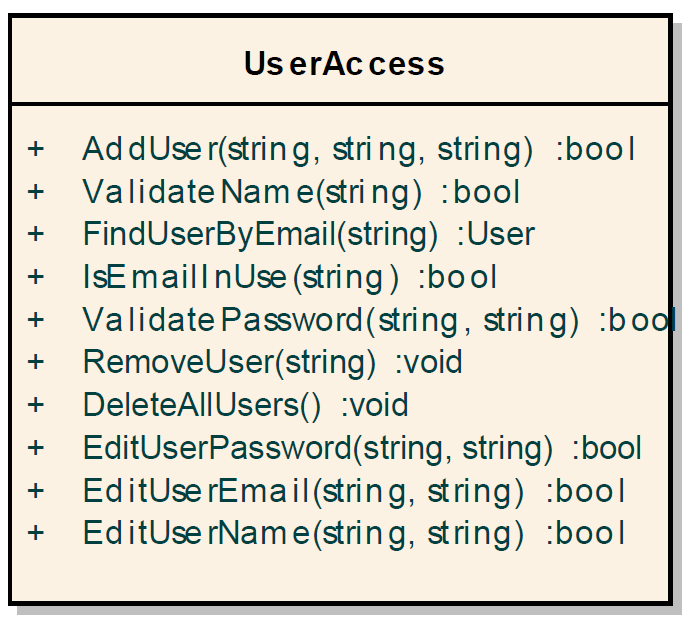
\includegraphics[width=0.4\linewidth]{figs/implementering/UserAccessClass.PNG}
\caption{Klassen UserAccess}
\label{fig:UserAccessClass}
\end{figure}


\paragraph{Metodebeskrivelser}
I dette afsnit findes metodebeskrivelser for klassen \textit{UserAccess}.

\subparagraph{AddUser}\

\textit{bool AddUser(string fullname, string email, string password)}

Står for at indsætte en user i databasen. Metoden kalder IsEmailInUse samt ValidateName før der oprettes et database kontekst objekt af typen DataBaseContext. På Kontekstobjektets DbSet<User> property kaldes Add metoden med den nye User som parameter. Herefter gemmes den nye User i databasen ved at kalde SaveChanges metoden på kontekstobjektet. AddUser returnerer false hvis der er fejl i enten check på email eller fullname. Hvis det lykkes at tilføje brugeren til databasen returneres true. Se metodens sekvensdiagram på figur~\ref{fig:adduser}

\begin{figure}[h]
\centering
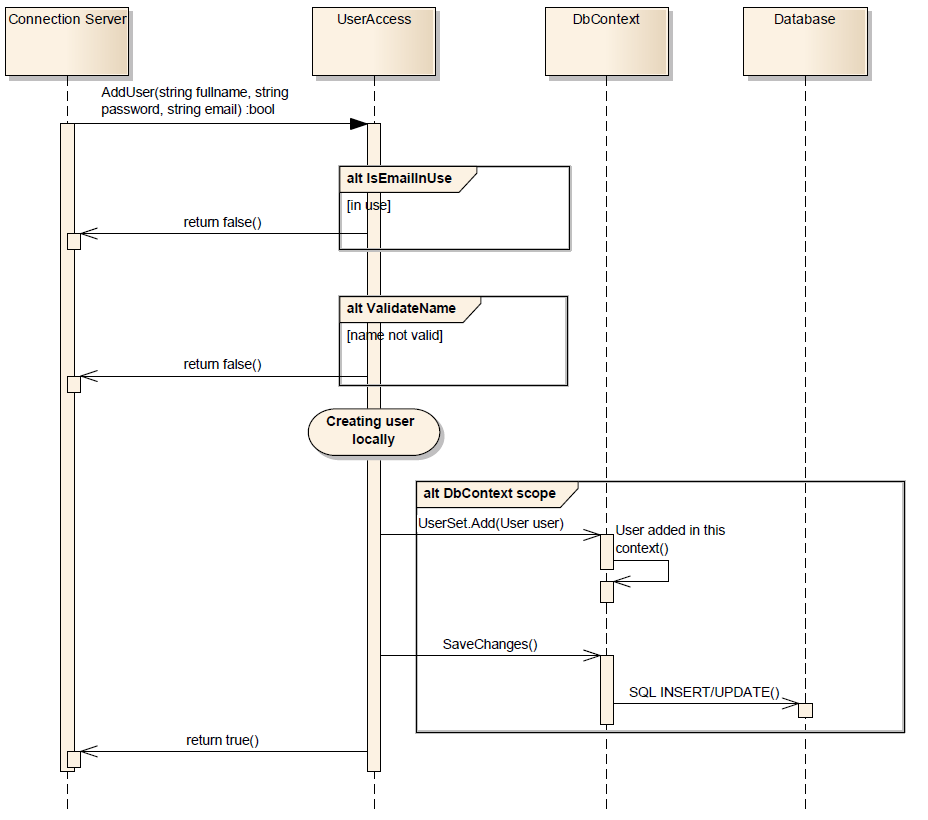
\includegraphics[width=\linewidth]{figs/dbSeq/adduser.PNG}
\caption{Sekvensdiagram for Metoden AddUser}
\label{fig:adduser}
\end{figure}


\subparagraph{FindUserByEmail}\

\textit{User FindUserByEmail(string email)}

Søger i databasen efter en User med den email der angives som parameter. Det må ikke eksistere flere brugere med samme email i databasen. Søgningen udføres med et LINQ statement på databasekonteksten. Se kodeudsnit~\ref{code:finduser}. Metoden returnerer den fundne User, med mindre der kastes en exception.
Se metodens sekvensdiagram på figur~\ref{fig:findUserByEmail}.

\begin{lstlisting}[caption=Kodeudsnit fra metoden FindUserByEmail, label=code:finduser]
...
using (var db = new DatabaseContext())
{
	var searchByEmail = from search in db.UserSet
			where search.Email.Equals(email)
			select search;

	if (searchByEmail.Count() > 1) throw new    	MultipleOccourencesOfEmailWasFoundException();
	if (searchByEmail.Count() == 0) throw new UserNotFoundException();

	foundUser = searchByEmail.First();
}
...	
\end{lstlisting}


\begin{itemize}
	\item \textit{MultipleOccourencesOfEmailWasFoundException()} - Sikkerhedsforanstaltning ved forekomst af flere ens emails.
	\item \textit{UserNotFoundException()} - Kastes hvis der ikke findes en bruger med den angivne email addresse i databasen.
\end{itemize}

\begin{figure}[h]
\centering
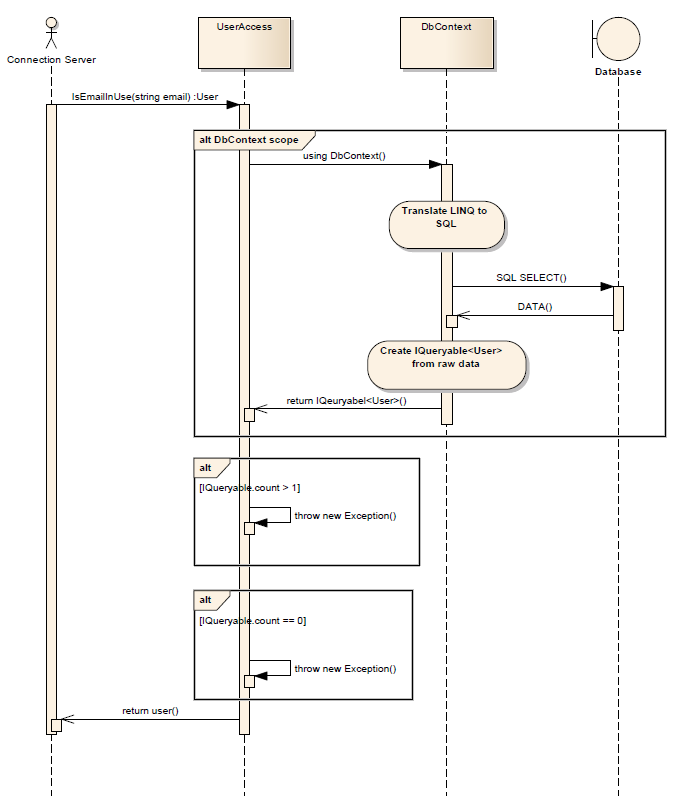
\includegraphics[width=\linewidth]{figs/dbSeq/findUserByEmail.PNG}
\caption{Sekvensdiagram for metoden FindUserByEmail}
\label{fig:findUserByEmail}
\end{figure}


\subparagraph{IsEmailInUse}\

\textit{bool IsEmailInUse(string email)}

Laver en LINQ query på databasekontekst objektet og checker om der findes en mailadresse i databasen der matcher, den som er givet med som parameter. Metoden returnerer false hvis mailaddressen ikke er i brug, og true hvis den er.

I sekvensdiagrammet på figur~\ref{fig:isEmailInUse}, kan det se hvordan en email checkes.

\begin{figure}[h]
\centering
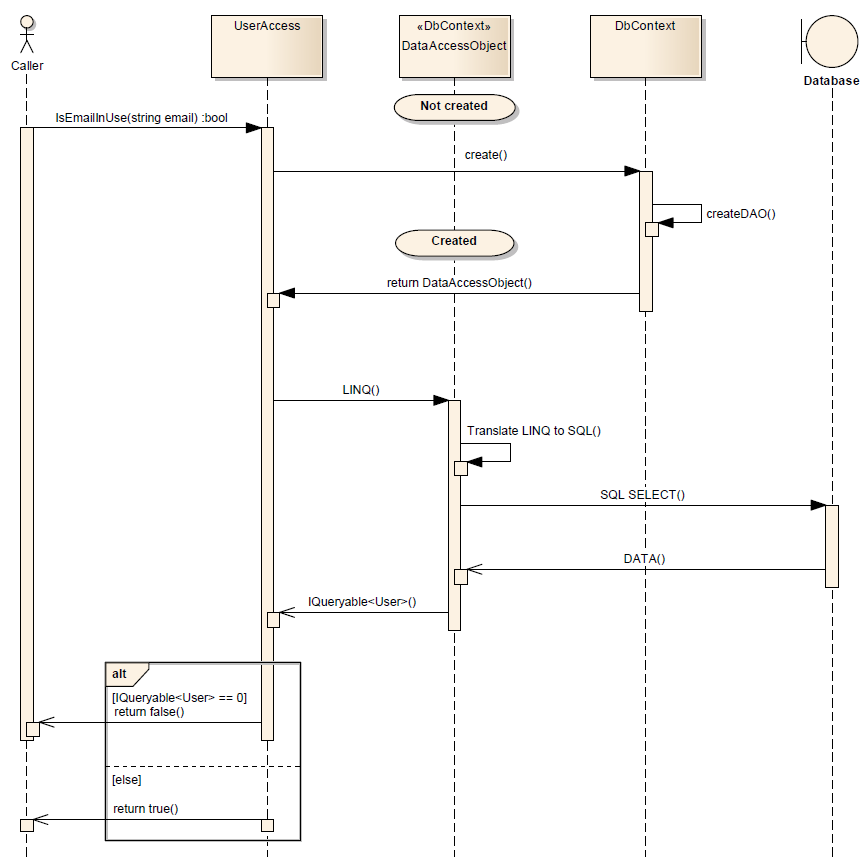
\includegraphics[width=0.7\linewidth]{figs/dbSeq/isEmailInUse.PNG}
\caption{Sekvensdiagram for metoden IsEmailInUse}
\label{fig:isEmailInUse}
\end{figure}


\subparagraph{ValidatePassword}\

\textit{bool ValidatePassword(string email, string password);}
Når der er brug for at validere en brugers password kaldes denne funktion. Den bruges eksempelvis når en bruger ønsker at logge ind på systemet. Se metodens sekvens diagram på figur~\ref{fig:validatePassword}
	
\begin{figure}[h]
\centering
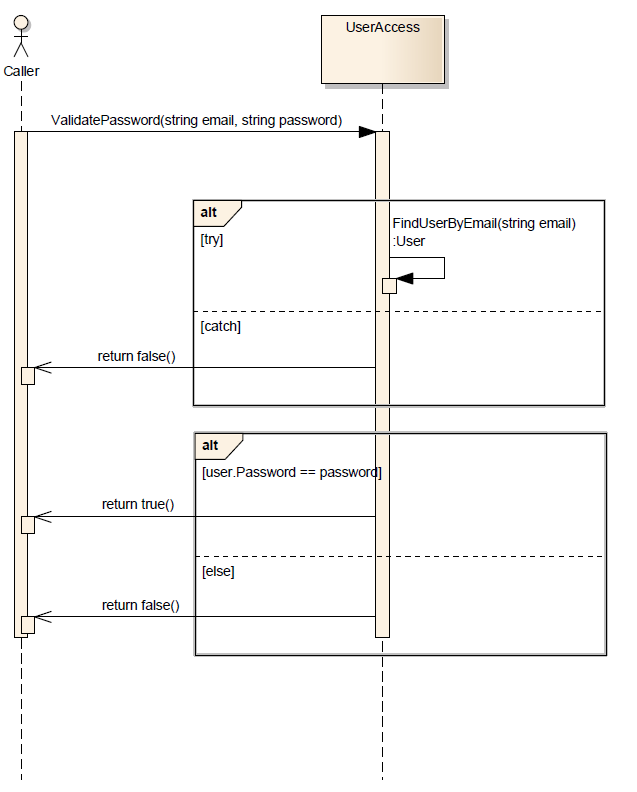
\includegraphics[width=0.7\linewidth]{figs/dbSeq/validatePassword.PNG}
\caption{Sekvensdiagram for metoden ValidatePassword}
\label{fig:validatePassword}
\end{figure}


\subparagraph{RemoveUser}\

\textit{void RemoveUser(string email)}

Checker først om en bruger med email findes.
Laver en LINQ query på databasekontekst objektet. Og finder den pågældende bruger.
Brugeren fjernes ved at kalde \textit{db.UserSet.Remove(user)} på kontekstobjektets UserSet property.

\begin{figure}[h]
\centering
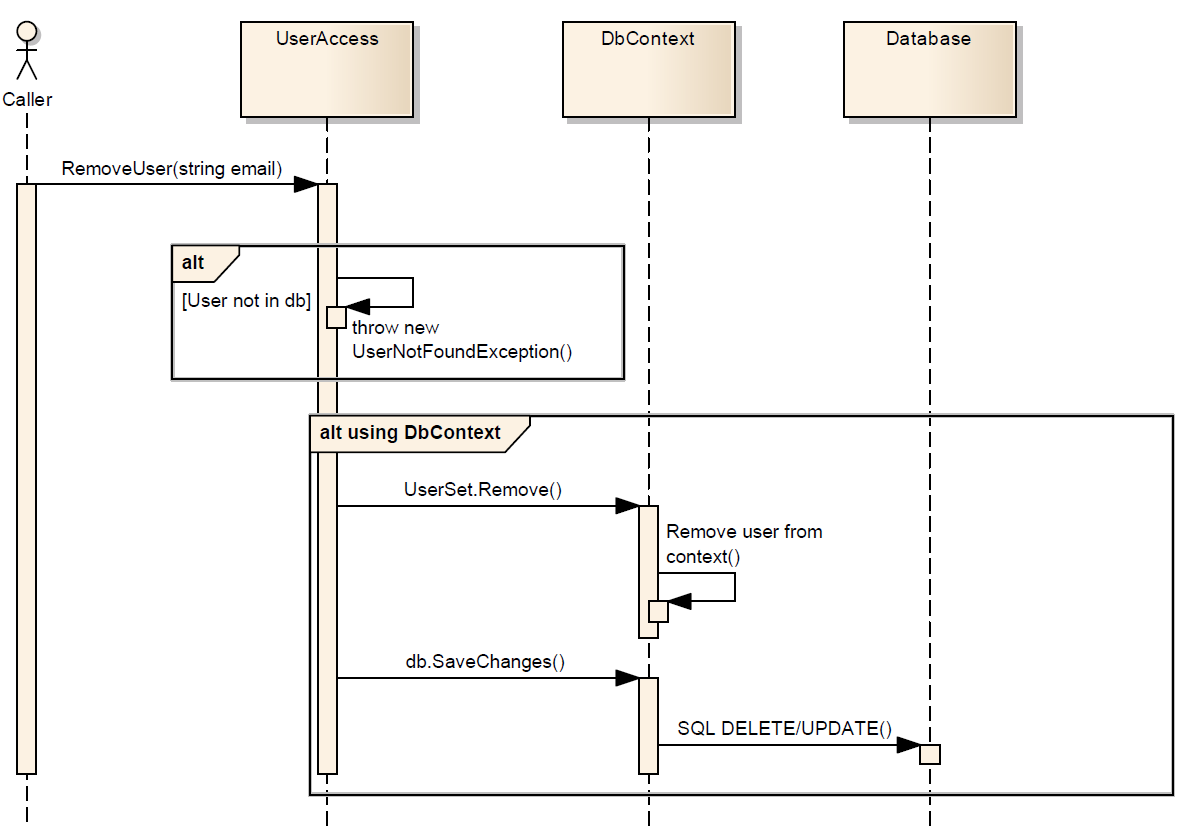
\includegraphics[width=0.7\linewidth]{figs/dbSeq/removeUser.PNG}
\caption{Sekvensdiagram for metoden RemoveUser}
\label{fig:removeUser}
\end{figure}


\subparagraph{DeleteAllUsers}\

\textit{void DeleteAllUsers()}

Bruges kun til systemtest og under udvikling.
Sletter alle brugere i databasen. Dette gøres ved at eksekvere en SQL kommando direkte på databasen. 

\begin{lstlisting}[caption=SQL injection på databasen ved sletning af brugere, label=sqlDeleteUsers]
...
using (var db = new DatabaseContext())
{
	db.Database.ExecuteSqlCommand("DELETE [UserSet]");
}
...	
\end{lstlisting}

\subparagraph{EditUserPassword}\

\textit{bool EditUserPassword(string email, string newPassword)}

Gør det muligt for en bruger at ændre sit password. Metoden står derudover for at sikre at det nye password ikke er en tom streng. User entitetens password property ændres gennem databasekonteksobjektet, hvorefter ændringen gemmes på databasen.
Metoden returnerer true med mindre der findes en uoverensstemmelse med enten password eller email.

\subparagraph{EditUserEmail}\

\textit{bool EditUserEmail(string email, string newEmail)}

Gør det muligt or en bruger at ændre sin email. Dette gøres gennem databasekontekst objektet. Når emailen er ændret skal brugeren benytte sig af den nye email ved et system login. \textit{Find()} metoden kaldes på kontekstobjektets UserSet property, med den ønskede brugers primærnøgle, \textit{Id}, hvorefter den pågældende User returneres. Se kodeudsnit \ref{code:idef} for eksempel på brugen af primær nøgler i entity frameworket.

\begin{lstlisting}[caption=EditUserEmail - brug af primær nøgler i Entity Framework,label=code:idef]
public bool EditUserEmail(string email, string newEmail)
{
	...
	using (var db = new DatabaseContext())
	{
		var original = db.UserSet.Find(FindUserByEmail(email).Id);
		if (original != null)
			{
				original.Email = newEmail;
				db.SaveChanges();
			}
	}
	return true;
}

\end{lstlisting}

\subparagraph{EditUserName}\

\textit{bool EditUserName(string email, string newName)}
Selvom der ikke findes en user story der ønsker funktionalitet til at ændre en bruger/User's navn, er der skrevet ekstra funktionalitet dertil. Dette er gjort for at fremtidssikre data access laget.

Se sekvensdiagrammet på figur~\ref{fig:editUserName}

\begin{figure}[h]
\centering
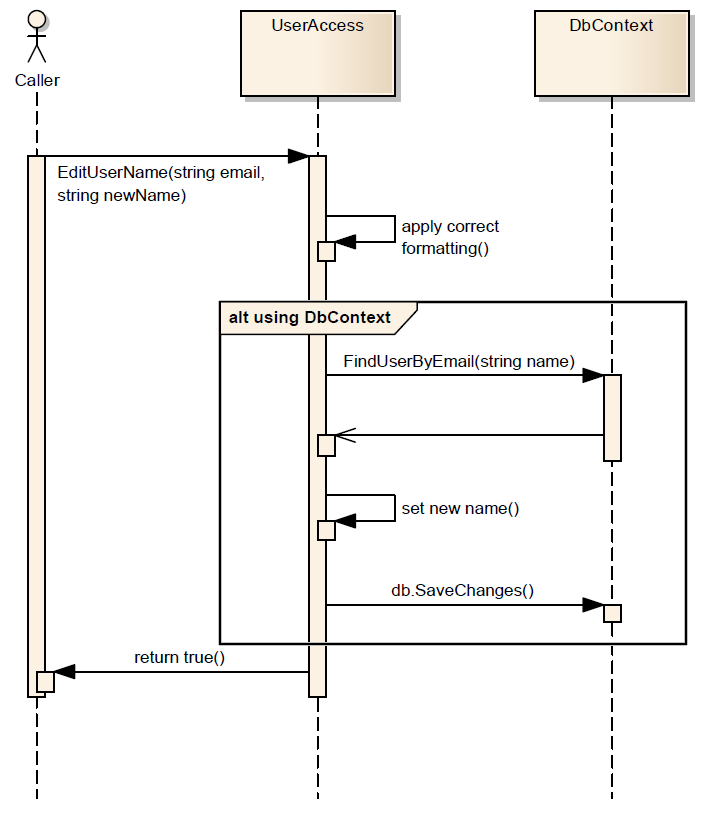
\includegraphics[width=0.7\linewidth]{figs/dbSeq/editUserName.PNG}
\caption{Sekvensdiagram for metoden EditUserName}
\label{fig:editUserName}
\end{figure}


\paragraph{Properties}\